\DocumentMetadata{
    lang=en-US,
    tagging=on,
    pdfversion=2.0,
    pdfstandard=ua-2,
    tagging-setup={math/setup=mathml-SE},
    colorprofiles={
        A = sRGB.icc, %or longer GTS_PDFA1 = sRGB.icc
        X = sRGB.icc,
        ISO_PDFE1 = sRGB.icc
    }
}

\documentclass{article}
\usepackage{notes}
\usepackage{standalone}

\begin{document}

\documentclass{article}
\usepackage{notes}

\begin{document}

\markright{Author: Silas Mitchell} % first page mark

\section{Chapter 1}
\subsection{Preliminaries}

This course assumes familiarity with basic arithmetic and algebraic operations.

There are several number systems that will be of interest throughout the course.
\begin{definition}{(Number systems)}{def:number_systems}
    \begin{itemize}
        \item Natural numbers: $\N=\{1,2,3,4,...\}$
        \item ``Whole" numbers: $W=\N\cup\{0\}=\{0,1,2,3,4,....\}$
        \item Integers: $\Z=\{...,-3,-2,-1,0,1,2,3,...\}$
        \item Rational numbers: $\Q=\left\{\frac{a}{b}:a,b\in\Z,b\neq0\right\}$
        \item Real numbers: informally, any number that can be expressed as a decimal. Denoted $\R$
        \item Irrational numbers: any real number which is not also a rational number
    \end{itemize}
\end{definition}

The book's terminology of ``whole numbers" is not standard, and conventions vary as to whether the natural numbers should start at 0 or at 1. Therefore, I will refer to the positive integers $\{1,2,3,...\}$ and the nonnegative integers $\{0,1,2,3,...\}$ instead.

\subsection{Visualizing and graphing data}
\subsubsection{One-variable data}

One variable data comes in the form of a list of numbers.

Given a set of one-variable data, we may represent it visually on a number line, or find various properties of the data. 

\begin{definition}{(Size-related properties of data)}{def:mim_max_range}
    \begin{itemize}
        \item Minimum: smallest value in the data set
        \item Maximum: largest value in the data set
        \item Range: difference between the minimum and maximum
    \end{itemize}
\end{definition}

\begin{definition}{(Mode)}{def:mode}
    The value that appears most frequently in the data set. (This value is not strictly unique, since we could have multiple values appear at the same frequency.)
\end{definition}

\begin{definition}{(Mean)}{def:mean}
    Also known as average. To take the average of $n$ numbers, add them all and then divide this total by $n$.
\end{definition}

\begin{definition}{(Median)}{def:median}
    Sort the list of data from smallest to largest. If there is an odd number of data points, then the mode is the middle one. Otherwise, take the average of the middle two.
\end{definition}

\begin{example}{(Textbook 1.2 ex 1)}{ex:1.2.1}
    The following table lists the low temperature, $T$, in degrees Fahrenheit that occured in Minneapolis, Minnesota for 6 consecutive nights:
    \begin{center} \tagpdfsetup{table/header-columns={1}}
    \begin{tabular}{|c|c|c|c|c|c|c|}\hline
        $T$ & $-12$ & $-4$ & $-8$ & $21$ & $18$ & $9$ \\ \hline
    \end{tabular}\end{center}
    \begin{enumerate}
        \item[(a)] Plot these temperatures on a number line.
        \item[(b)] Find the maximum and minimum of these temperatures.
        \item[(c)] Determine the mean of these six temperatures.
        \item[(d)] Find the median and interpret the result.
    \end{enumerate}
\end{example}
\begin{solution}
	\begin{enumerate}
        \item[(a)] $\quad$\\
        \begin{tikzpicture}[scale=.39,alt={number line with temperature data plotted}]
            \draw[<->, very thick] (-13.5,0) -- (22.5,0);
            \foreach \x in {-13,-8,...,22} {do
                \draw (\x,.2) -- (\x,-.2) node[anchor=north] {$\x$};
            }
            \filldraw (-12,0) circle (5pt);
            \filldraw (-4,0) circle (5pt);
            \filldraw (-8,0) circle (5pt);
            \filldraw (21,0) circle (5pt);
            \filldraw (18,0) circle (5pt);
            \filldraw (9,0) circle (5pt);
        \end{tikzpicture}
        \item[(b)] Maximum: 21\\ Minimum: -12
        \item[(c)] Mean: \[\frac{(-12)+(-4)+(-8)+21+18+9}{6}=\frac{24}{6}=4.\]
        \item[(d)] Median: First we put the data in increasing order: 
        \[-12,-8,-4,9,18,21.\]
        Since there is an even number of data points, we take the average of the middle two:
        \[\frac{-4+9}{2}=\frac{5}{2}.\]
        This means that half of the nights were warmer than $2.5^\circ$F, and half were colder.
    \end{enumerate}
\end{solution}

\begin{directions}
    Ask students if they have any questions before moving on.
\end{directions}

\subsubsection{Two-variable data}

Sometimes, there is a relationship between two pieces of data. We call this a relation.

\begin{definition}{(Ordered pair)}{def:ordered_pair}
    Suppose we have two related lists of data. An ordered pair, written $(x,y)$, is a pair of numbers where the first number $x$ comes from the first list and the second number $y$ comes from the second.
\end{definition}

\begin{definition}{(Relation)}{def:relation}
    A relation is a set of ordered pairs. We can also think of it as two lists of data which are related to each other.
\end{definition}

\begin{definition}{(Domain and range)}{def:relation_domain_range}
    \begin{itemize}
        \item The domain of a relation is the set of $x$ values from the relation (first components of the ordered pairs)
        \item The range of a relation is the set of $y$ values from the relation (second components of the ordered pairs)
    \end{itemize}
\end{definition}

\begin{example}{Textbook 1.2 ex 2}{ex:1.2.2}
    A physics class measured the time $y$ that it takes for an object to fall $x$ feet, as shown in the following table. The object was dropped twice from each height.
    \begin{center} \tagpdfsetup{table/header-columns={1}}
    \begin{tabular}{|r|c|c|c|c|} \hline
        $x$ (feet) & $20$ & $20$ & $40$ & $40$ \\ \hline
        $y$ (seconds) & $1.2$ & $1.1$ & $1.5$ & $1.6$ \\ \hline
    \end{tabular}\end{center}
    \begin{problem}
        \item Express the data as a relation $S$.
        \item Find the domain and range of $S$.
    \end{problem}
\end{example}
\begin{solution}
    \begin{problem}
        \item A relation is a list of ordered pairs, so we need to list all of the ordered pairs from the table. Each column gives us an ordered pair. Thus, \[S=\bigl\{(20,1.2),(20,1.1),(40,1.5),(40,1.6)\bigr\}.\]
        \item The domain is the set of possible $x$ values: \[D(S)=\{20,40\}.\] The range is the set of possible $y$ values: \[R(S)=\{1.2,1.1,1.5,1.6\}.\]
    \end{problem}
\end{solution}

When we have two-variable data, it can be useful to represent this visually.
\begin{definition}{(Cartesian coordinates)}{def:cartesian_coordinates}
    To graph, we use the $xy$-plane, also called Cartesian coordinates. The horizontal axis is called the $x$-axis, and the vertical axis is the $y$-axis.
    \begin{center}\begin{tikzpicture}[scale=.4,alt={the $xy$-plane}]
        \draw[thick, <->] (-5,0) node[anchor=north east] {Negative $x$-axis} -- (5,0) node[anchor=north west] {$x$-axis};
        \draw[thick, <->] (0,-5) node[anchor=north east] {Negative $y$-axis} -- (0,5) node[anchor=south west] {$y$-axis};
        \filldraw (2,3) circle (2pt) node[anchor=north] {$(x,y)$};
        \draw (2,-.1) node[anchor=north] {$x$} -- (2,.1);
        \draw (-.1,3) node[anchor=east] {$y$} -- (.1,3);
    \end{tikzpicture}\end{center}
\end{definition}

\begin{definition}{(Graphing two-variable data)}{def:graphing_2d}
    \begin{itemize}
        \item Graphing each point in a relation gives a scatterplot
        \item If a relation only has one point per $x$ value, we can make a line graph by connecting consecutive points in the scatterplot with line segments
    \end{itemize}
\end{definition}

\begin{example}{(Textbook 1.2 ex 3)}{ex:1.2.3}
    Complete the following for the relation \[S=\bigl\{(5,10),(5,-5),(-10,10),(0,15),(-15,-10)\bigr\}.\]
    \begin{problem}
        \item Find the domain and range of the relation.
        \item Determine the maximum and minimum of the $x$-vales and then of the $y$-values.
        \item Label appropriate scalse on the $x-$ and $y$-axes.
        \item Plot the relation as a scatterplot.
    \end{problem}
\end{example}
\begin{solution}
    \begin{problem}
        \item The domain is the set of $x$ values: $D=\{5,-10,0,-15\}$.\\ The range is the set of $y$ values: $R=\{10,-5,15,-10\}$.
        \item \;\vspace{-15pt}\begin{center} \tagpdfsetup{table/header-rows={1}}\tagpdfsetup{table/header-columns={1}}
        \begin{tabular}{c|cc}
            & Maximum & Minimum \\ \hline
            $x$-values & $5$ & $-15$ \\
            $y$-values & $15$ & $-10$
        \end{tabular}\end{center}
        \item The axes need to cover the full $x$ and $y$ range. It's also customary to include slightly more on each end. Since the data is all multiples of 5, we might have each tick represent 5. We can have the $x$ axis range from $-20$ to $10$, and the $y$ axis range from $-15$ to $20$.
        \item \;\vspace{-15pt} \begin{center}\begin{tikzpicture}[alt={graph of the relation}]
            \draw[very thick, <->] (-2,0) node[anchor=north east] {$-20$} -- (1,0) node[anchor=north west] {$10$};
            \draw[very thick, <->] (0,-1.5) node[anchor=north] {$-15$} -- (0,2) node[anchor=south west] {$20$};
            \draw[gray, thin, step=.5] (-2,-1.5) grid (1,2);
            \filldraw (.5,1.0) circle (2pt);
            \filldraw (.5,-.5) circle (2pt);
            \filldraw (-1.0,1.0) circle (2pt);
            \filldraw (0,1.5) circle (2pt);
            \filldraw (-1.5,-1.0) circle (2pt);
        \end{tikzpicture}\end{center}
    \end{problem}
    Note that we can't turn this into a line graph because there are multiple points with the same $x$ coordinate, so it isn't clear which points we would consider consecutive.
\end{solution}

\subsubsection{Midpoint between points}

If we have two data points and want to find the point halfway between them, we can use the midpoint formula. 

\begin{formula} {(Midpoint formula)}{formula:midpoint}
    The midpoint of the line segment between points\((x_1,y_1)\) and \((x_2,y_2)\) is the point \[\left(\frac{x_1+x_2}{2},\frac{y_1+y_2}{2}\right).\] In other words, its coordinates are the average of the coordinates of the two endpoints.
\end{formula}

\begin{example}{(Textbook 1.2 ex 7)}{ex:1.2.7}
    Find the midpoint of the line segment connecting the points \((6,-7)\) and \((-4,6)\).
\end{example}
\begin{solution}
    We have \((x_1,y_1)=(6,-7)\) and \((x_2,y_2)=(-4,6)\). Plugging these into the midpoint formula, we get
    \begin{align*}
        \left(\frac{x_1+x_2}{2},\frac{y_1+y_2}{2}\right) &= \left(\frac{6+(-4)}{2},\frac{-7+6}{2}\right) \\
        &= \left(\frac{2}{2},\frac{-1}{2}\right) \\
        &= \left(1,-\frac{1}{2}\right).
    \end{align*}
\end{solution}

This can be useful for making estimates in real-world scenarios.

\begin{example}{}{ex:1.2_linear_interpolation}
    Suppose the weather forecast calls for 2 inches of snow to fall between midnight and 6 am. Use the midpoint formula to estimate how much snow will have fallen by 3 am.
\end{example}
\begin{solution}
    First, we need to find the endpoints. At midnight, it has been 0 hours since snow started falling, and 0 inches of snow have fallen. We can interpret this as the point \((0,0)\). At 6 am, it has been 6 hours since snow started falling, and 2 inches have fallen; this gives us the point \((6,2)\).

    Now we plug the points into the formula:
    \begin{align*}
        \left(\frac{x_1+x_2}{2},\frac{y_1+y_2}{2}\right) &= \left(\frac{0+6}{2},\frac{0+2}{2}\right) \\
        &=\left(\frac{6}{2},\frac{2}{2}\right) \\
        &=(3,1).
    \end{align*}
    Back in the original context, this means that 3 hours after the snowfall starts, we expect there to be 1 inch of snow on the ground.
\end{solution}

\subsubsection{Distance between points}

Sometimes, we want to be able to find the distance between two points on the plane. 

We can compute the vertical and horizontal distances between the points as the difference between the $y$ coordinates and $x$ coordinates, respectively. Then the Pythagorean theorem allows us to find the distance between the two points:

\begin{formula}{(Pythagorean Theorem)}{formula:pythag}
    Let \(\triangle ABC\) be a right triangle with sides $a,b,c$. If \(c\) is the hypotenuse, then we have \[a^2+b^2=c^2.\] Taking the square root of both sides, we get the relationship \[c=\sqrt{a^2+b^2}.\]
\end{formula}
\begin{definition}{(Distance between points)}{def:distance_formula}
    \begin{center}\begin{tikzpicture}[scale=.5,alt={example of right triangle made from two points on the plane}]
        \draw[thick, <->] (-1,0) -- (6,0);
        \draw[thick, <->] (0,-1) -- (0,5);
        \draw[dotted] (1,4) node[anchor=south] {$\scriptstyle (x_1,y_1)$} -- (1,1) -- (5,1) node[anchor=west] {$\scriptstyle (x_2,y_2)$};
        \draw (1,4) -- (5,1);
    \end{tikzpicture}
    % alt={Drawing of right triangle with sides parallel to axes given by two points in the plane}
    \end{center}
    The distance between $(x_1,y_1)$ and $(x_2,y_2)$ is the length of the hypotenuse of a triangle whose sides are the change in $x$, $x_2-x_1$, and the change in $y$, $y_2-y_1$. Thus it is \[\sqrt{(x_2-x_1)^2+(y_2-y_1)^2}\]
\end{definition}

\begin{example}{}{ex:1.2_distance_points}
    Find the distance between the points $(1,4)$ and $(5,1)$.
\end{example}
\begin{solution}
    We have \begin{align*}(x_1,y_1)&=(1,4) \\ (x_2,y_2)&=(5,1).\end{align*} Then we plug these into the formula and simplify to find the distance:
    \begin{align*}
        \sqrt{(x_2-x_1)^2+(y_2-y_1)^2}&=\sqrt{(5-1)^2+(1-4)^2}\\
        &=\sqrt{(4)^2+(-3)^2}\\
        &=\sqrt{16+9}\\
        &=\sqrt{25}\\
        &=5.
    \end{align*}
    Therefore, the two points are 5 units apart.
\end{solution}

\begin{example}{(Textbook 1.2 ex 6)}{ex:1.2.6}
    Suppose that at noon car $A$ is traveling south at 20 miles per hour and is located 80 miles north of car $B$. Car $B$ is traveling east at 40 miles per hour.
    \begin{problem}
        \item Let $(0,0)$ be the initial coordinates of car $B$ in the $xy$-plane, where units are in miles. Plot the location of each car at noon and at 1:30 pm.
        \item Approximate the distance between the cars at 1:30 pm.
    \end{problem}
\end{example}
\begin{solution}
    \begin{problem}
        \item First we need to figure out where the points are.
        
        We know that car $B$ is at $(0,0)$ at noon, and $A$ is 80 miles north of $B$. Therefore, car $A$ is at $(0,80)$ at noon.

        Between noon and 1:30 pm is 1.5 hours. Car $A$ is moving 20 mph south, so travels $20\frac{\text{miles}}{\text{hour}}\cdot 1.5\text{ hours}=30$ miles south. Therefore, car $A$ is at $(0,50)$ at 1:30 pm.

        Car $B$ is moving 40 mph east, so travels $40\frac{\text{miles}}{\text{hour}}\cdot1.5\text{ hours}=60$ miles east. Therefore, car $B$ is at $(60,0)$ at 1:30 pm.
        \begin{center}\begin{tikzpicture}[alt={plot of the locations of the cars}]
            \draw[thick, <->] (-1,0) -- (5,0);
            \draw[thick, <->] (0,-1) -- (0,5);
            \filldraw (0,0) circle (2pt) node[anchor=north west] {$B$ at noon; $(0,0)$};
            \filldraw (0,4) circle (2pt) node[anchor=west] {$A$ at noon; $(0,80)$};
            \filldraw (3,0) circle (2pt) node[anchor=south] {$B$ at 1:30; $(60,0)$};
            \filldraw (0, 2.5) circle (2pt) node[anchor=west] {$A$ at 1:30; $(0,50)$};
        \end{tikzpicture}\end{center}
        \item We need to find the distance between the points $(x_1,y_1)=(0,50)$ and $(x_2,y_2)=(60,0)$. Plugging these into the formula, we get
        \begin{align*}
            \sqrt{(x_2-x_1)^2+(y_2-y_1)^2}&=\sqrt{(60-0)^2+(0-50)^2}\\
            &=\sqrt{(60)^2+(-50)^2}\\
            &=\sqrt{3600+2500}\\
            &=\sqrt{6100}\\
            &=10\sqrt{61}.
        \end{align*}
    \end{problem}
\end{solution}

\subsubsection{Circles}

\begin{directions}
    Ask students how to characterize a circle.
\end{directions}
\begin{definition}{(Circle)}{def:circle}
    A circle is the set of all points at a set distance from a fixed center. We call the distance from each point to the center the radius of the circle.

    Denote the center by the point \((h,k)\) and the radius by \(r\).
\end{definition}

The distance equation tells us that every point \((x,y)\) on the circle with radius \(r\) and center \((h,k)\) satisfies \[\sqrt{(x-h)^2+(y-k)^2}=r.\] Squaring both sides gives us the standard equation of a circle:

\begin{formula} {(Standard equation for a circle)}{eqn:circle_standard}
    The equation for the circle with radius \(r\) and center \((h,k)\) is \[(x-h)^2+(y-k)^2=r^2.\] % In the special case that \((h,k)=(0,0)\) then we can simplify this to \(x^2+y^2=r^2\).
\end{formula}

\begin{example}{}{ex:1.2_circle_data_to_eqn}
    Write the equation for a circle with radius 5 and center \((1,0)\).
\end{example}
\begin{solution}
    We have \(r=5\) and \((h,k)=(1,0)\). Plugging this into the standard form, we get \[(x-1)^2+(y-0)^2=5^2,\] or equivalently \[(x-1)^2+y^2=25.\]
\end{solution}

\begin{example}{(Textbook 1.2 ex 9)}{ex:1.2.9}
    Find the center and radius of the circle with the given equation. Graph each circle.
    \begin{problem}
        \item \(x^2+y^2=9\)
        \item \((x-1)^2+(y+2)^2=4\)
    \end{problem}
\end{example}
\begin{solution}
    \begin{problem}
        \item Since \(x=x-0\) and \(y=y-0\), we can equivalently write this as \((x-0)^2+(y-0)^2=4\). Then the center is \((-0,-0)=(0,0)\) and the radius is \(\sqrt{9}=3\).
        \item The center is \((-(-1),-2)=(1,-2)\) and the radius is \(\sqrt{4}=2\).
    \end{problem}
    \begin{center} \tagpdfsetup{table/tagging=presentation}
    \begin{tabular}{cc}
    \begin{tikzpicture}[scale=.6,alt={graph of cirle a}]
        \draw[very thick,<->] (-2.1,0) -- (2.1,0) node[anchor=west] {\(x\)};
        \draw[very thick,<->] (0,-2.1) -- (0,2.1) node[anchor=south] {\(y\)};
        \draw[gray, thin,step=.5] (-2,-2) grid (2,2);
        \filldraw (0,0) circle (2pt);
        \draw (0,0) circle (1.5);
    \end{tikzpicture}
    &
    \begin{tikzpicture}[scale=.8, alt={graph of circle b}]
        \draw[very thick,<->] (-1.1,0) -- (2.1,0) node[anchor=west] {\(x\)};
        \draw[very thick,<->] (0,-2.6) -- (0,.6) node[anchor=south] {\(y\)};
        \draw[gray, thin,step=.5] (-1,-2.5) grid (2,.5);
        \filldraw (.5,-1) circle (2pt);
        \draw (.5,-1) circle (1);
    \end{tikzpicture}
    \end{tabular}\end{center}
\end{solution}

Sometimes, we might know the center and one point on the circle. Then we can find the radius by using the distance formula to determine the distance between the two points.

We might also be given two endpoints of a diameter of a circle. Then the center is the midpoint, which we can find with the midpoint formula, and the radius can be found using the distance formula with one of the endpoints and the center we found.

\subsubsection{Completing the square}

Whenever we have a term like \((x-h)^2=(x-h)(x-h)\), we can use FOIL to multiply it out.

\begin{directions}
    Ask students if they remember what FOIL is. Remind students that FOIL stands for First, Outer, Inner, Last and demonstrate multiplying out \((x-h)^2=x^2-2xh+h^2\).
\end{directions}

In particular, we can manipulate the equation of a circle by multiplying out the squared terms to get something in the form of a general equation of a circle.
\begin{formula}{(General equation of a circle)}{eqn:circle_general}
    The general equation of a circle has the form \[x^2+ax+y^2+by=c\] for some constants \(a,b,c\).
\end{formula}

When we want to determine the center and/or radius of a circle given its equation in general form, we need to use a process called completing the square.

\begin{process}{Completing the square}{formula:complete_the_square}
    We start with an expression of the form \(x^2+ax\) and want to get an expression resembling \((x+b)^2\). Observe that \((x+\frac{a}{2})^2=x^2+ax+\left(\frac{a}{2}\right)^2\). Therefore, $x^2+ax=(x+\frac{a}{2})^2-\left(\frac{a}{2}\right)^2$.

    We call this completing the square because the extra term \(\left(\frac{a}{2}\right)^2\) allows us to make a perfect square:
    \todo{add pic of completing the square}
    \begin{center}\begin{tikzpicture}[alt={visual for completing the square}]
        
    \end{tikzpicture}\end{center}
    \vspace{2in}
\end{process}

\begin{example}{}{ex:1.2_complete_the_square}
    Complete the square with the following equation: \(y^2-6y=18\).
\end{example}
\begin{solution}
    In this equation, we use the variable \(y\) instead of \(x\); however, the process still works in exactly the same way. We have \(a=-6\), so get that \(y^2-6y=(y+\frac{-6}{2})^2-(-6/2)^2\). Substituting this into the original equation, we have $(y-3)^2+9=18$, which turns into $(y-3)^3=9$ when we move all constant terms to the right.
\end{solution}

\begin{directions}
    Ask students if this makes sense. If not, do another example.
\end{directions}

\begin{example}{(Textbook 1.2 ex 12)}{ex:1.2.12}
    Find the center and radius of the circle given by \(x^2+4x+y^2-6y=5\).
\end{example}
\begin{solution}
    First, we need to transform the equation into standard form. We will do this by completing the square with both the \(x\) terms and the \(y\) terms.

    The \(x\) terms are \(x^2+4x\). Completing the square, we get \(x^2+4x=(x+\frac{4}{2})^2-\left(\frac{4}{2}\right)^2\).

    The \(y\) terms are \(y^2-6y\). Completing the square, we get \(y^2-6y=(y+\frac{-6}{2})^2-\left(\frac{-6}{2}\right)^2\).

    Substituting both of these into the original equation and simplifying, we get
    \begin{align*}
        (x^2+4x)+(y^2-6y)&=5\\
        ((x+2)^2-4)+((y-3)^2-9)&=5\\
        (x+2)^2+(y-3)^2-4-9&=5\\
        (x+2)^2+(y-3)^2&=5+4+9=18.
    \end{align*}

    Now we can find the center and radius. The center is \((-2,3)\) and the radius is \(\sqrt{18}\).
\end{solution}

\end{document}

% uncomment this to compile individual section
% \DocumentMetadata{
%     lang=en-US,
%     tagging=on,
%     pdfversion=2.0,
%     pdfstandard=ua-2,
%     tagging-setup={math/setup=mathml-SE},
%     colorprofiles={
%         A = sRGB.icc, %or longer GTS_PDFA1 = sRGB.icc
%         X = sRGB.icc,
%         ISO_PDFE1 = sRGB.icc
%     }
% }

\documentclass{article}
\usepackage{notes}

\begin{document}

\setcounter{section}{1}
\setcounter{subsection}{2}

\subsection{Functions and Their Representations}

\subsubsection{What is a function?}

\begin{definition}{(Function)}{def:function}
    A function is a process that receives inputs and produces outputs. For each input, the function must give exactly one output.

    We write ``$f(x)=y$'' to mean ``on input $x$, the function $f$ returns output $y$''.

    Alternatively, a function is a relation where every element of the domain corresponds to exactly one element of the range. All functions are relations, but not all relations are functions (see \ref{ex:1.2.3}).
\end{definition} 

Let's consider an example of a function. There is a relationship between distance from a lightning strike and seconds between seeing the lightning and hearing the thunder. We could have a function that takes the number of seconds between the lightning and thunder, and returns the distance in miles from the lightning strike.

\begin{directions}
    Write on board:\\
    Example function: takes seconds between lightning and thunder, and returns distance in miles to the lightning strike.
\end{directions}

\begin{definition}{(Representations of functions)}{def:function_representations}
    There are many ways to represent the data of a function.
    \begin{itemize}
        \item Verbal representation: verbally describe the computation of a function.\\ Ex: ``divide $x$ by 5''.
        \item Numerical representation: table of values. Since these generally contain only a portion of the possible domain of the function, we call it a partial numerical representation.\\ Ex:
            \begin{center} \tagpdfsetup{table/header-columns={1}}
            \begin{tabular}{|c|c|c|c|c|c|} \hline
                 $\mathbf{x}$ & $0$ & $5$ & $10$ & $15$ & $20$ \\ \hline
                 $\mathbf{y}$ & $0$ & $1$ & $2$ & $3$ & $4$ \\ \hline
            \end{tabular}\end{center}
        \item Graphical representation: a plot of ordered pairs belonging to the relation.\\Ex:
        \begin{center}\begin{tikzpicture}[alt={graph}]
            \draw[very thick, <->] (-.2,0) -- (5.2,0) node[anchor=west] {$x$};
            \draw[very thick, <->] (0,-.2) -- (0,1.2) node[anchor=south] {$y$};
            \draw[<->] (-.1,-.02) -- (5.1,1.02);
            \foreach \x in {1,...,5} {
                \pgfmathsetmacro\y{int(\x*5)}
                \draw (\x,.1) -- (\x,-.1) node[anchor=north] {\y};
                \draw (.1,\x / 5) -- (-.1,\x / 5) node[anchor=east] {\tiny \x};
            }
        \end{tikzpicture}\end{center}
        \item Symbolic representation: a formula telling us what to evaluate for each input.\\Ex: $f(x)=\frac{x}{5}$
    \end{itemize}
\end{definition}

\begin{example}{(Textbook 1.3 ex 7)}{ex:1.3.7}
    When the relative humidity is less than $100\%$, air cools at $3.6^\circ F$ for every 1000-foot increase in altitude. Let $f$ be a function that computes this change in temperature for an increase in altitude of $x$ thousand feet, with domain $0\leq x\leq 6$. Represent $f$
    \begin{problem}
        \item verbally
        \item symbolically
        \item graphically
        \item numerically
    \end{problem}
\end{example}
\begin{solution}
    \begin{problem}
        \item Multiply the input, $x$, by $-3.6$ to get the change in temperature, $y$.
        \item $f(x)=-3.6x$
        \item \,\begin{center}\begin{tikzpicture}[scale=.6,alt={graph of the function from part b}]
            \draw[very thick,<->] (-0.2, 0) -- (6.2,0) node[anchor=west] {$x$};
            \draw[very thick,<->] (0,.2) node[anchor=south] {$y$} -- (0,-3.2);
            \foreach \x in {1,...,6} {
                \draw (\x,.1) -- (\x,-.1) node[anchor=north] {$\x$};
            }
            \foreach \y in {3.6,7.2,...,21.6} {
                \draw (.1,\y/-7.2) -- (-.1,\y/-7.2) node[anchor=east] {$-\y$};
            }
            \draw[<->] (-.1,-.05) -- (6.1,-3.05);
        \end{tikzpicture}\end{center}
        \item $\quad$\\ \vspace{-30pt}\begin{center}\begin{tabular}{|c|c|c|c|c|} \hline
            Increase in altitude (ft) & 0 & 1000 & 2000 & 3000 \\ \hline
            Change in temperature ($^\circ F$) & 0 & -3.6 & -7.2 & -10.8 \\ \hline
        \end{tabular}\end{center}
    \end{problem}
\end{solution}
% \includegraphics[width=6.5in]{Textbook_Mandatory_Examples/Exam1/1.3/1.3.7.png}

\begin{example}{(Textbook 1.3 ex 3)}{ex:1.3.3}
    The function \(f\) computes the revenue in dollars per unique user for different technology companies. This function is defined by \(f(A)=189,f(G)=24,f(Y)=8,f(F)=4\), where \(A\) is Amazon, $G$ is Google, $Y$ is Yahoo, and $F$ is Facebook.
    \begin{problem}
        \item Write $f$ as a set of ordered pairs.
        \item Give the domain and range of $f$.
        \item Interpret $f(A)=189$.
    \end{problem}
\end{example}
\begin{solution}
    \begin{problem}
        \item From $f(x)=y$, we get the ordered pair $(x,y)$. Therefore, we have \[f=\{(A,189), (G,24), (Y,8), (F,4)\}.\]
        \item Now that we have $f$ written as a list of ordered pairs, we can find the domain and range just like we did when working with relations.
        \begin{align*}
            D_f&=\{A,G,Y,F\}\\
            R_f&=\{189,24,8,4\}
        \end{align*}
        \item $f$ takes a company as input and returns the revenue in dollars per unique user. Therefore, $f(A)=189$ means Amazon receives \$189 in revenue per unique visitor.
    \end{problem}
\end{solution}

\subsubsection{Notating sets of real numbers}

For functions with finite domains, we can write the entire domain as a set. However, many functions have infinite domains, so we need more sophisticated ways to describe their domains.

Previously, we have notated everything as a set.

\begin{definition}{(Sets)}{def:set}
    A set is a collection of elements. We notate them surrounded by curly braces and separated by commas: $\{a,b,c\}$. The order of items within the braces does not matter; an item can only be in a set once (so repetitions do not matter).
\end{definition}

The first method we have is a refinement of the sets we were already using, and is called set builder notation.

\begin{definition}{(Set-builder notation)}{def:set_builder}
    The pattern for set builder notation is $\{x\in \text{[big set]}:\text{[conditions on $x$]}\}$. Sometimes, a pipe is used as a separator instead of a colon. If we don't specify the big set, then it typically means $x$ is a real number.
\end{definition}

\begin{example}{}{ex:set_builder}
    \begin{itemize}
        \item We can exclude specific values\\Ex: $\{x : x\neq 1,x\neq 2,x\neq 3\}$
        \item We can set a minimum or maximum value\\Ex: $\{x : x<-2\}$\\\phantom{Ex: }$\{x : x\geq 7\}$
        \item We can specify a range\\Ex: $\{x : \frac{1}{2}\leq x < 7\}$
        \item We can combine multiple different types of condition\\Ex: $\{x : x > 0, x\neq 1\}$
    \end{itemize}
\end{example}

The second tool we have is called interval notation. 

\begin{definition}{(Interval notation)}{def:interval_notation}
    Interval notation consists of the two endpoints of the interval written inside parentheses or square brackets, depending on whether each endpoint is included or not. A square bracket means that endpoint is included, and a parenthesis mean it is not. There are 4 possible cases:
    \begin{itemize}
        \item $a<x<b$ becomes $(a,b)$
        \item $a<x\leq b$ becomes $(a,b]$
        \item $a\leq x<b$ becomes $[a,b)$
        \item $a\leq x\leq b$ becomes $[a,b]$
    \end{itemize}
    If there is no lower endpoint, we write $-\infty$ (cases where $x<b$ or $x\leq b$). If there is no upper endpoint, we write $\infty$ (whenever $a<x$ or $a\leq x$). We always use parentheses with infinity.
\end{definition}

Sometimes, we may have sets that consist of two intervals.

\begin{definition}{(Union)}{def:union}
    The union of two sets is the set which consists of all elements from either set. It is denoted $\cup$.

    We can take the union of intervals, such as $(-\infty,-1)\cup[3,5]\cup(9,\infty)$.
\end{definition}

\subsubsection{Domain, range, and evaluation}

\begin{definition}{(Domain)}{def:domain}
    We think of the domain as the set of all valid inputs which make sense when plugged in. More formally, the domain of a function $f$ is the set of all real numbers for which its formula is defined. Sometimes we refer to this as the implied domain.
\end{definition}
\begin{example}{}{ex:domain_easy}
    \begin{itemize}
        \item $f(x)=x$: it makes sense to plug in any real number, so the domain is all real numbers.\\$\{x\in \R\}$ or $(-\infty,\infty)$
        \item $g(x)=\frac{1}{x}$: we can plug in any number except for 0, so the domain is everything but 0.\\$\{x:x\neq 0\}$ or $(-\infty,0)\cup(0,\infty)$
        \item $h(x)=\sqrt{3x}$: we can plug in any nonnegative number, so the domain is $x\geq 0$.\\$\{x:x\geq 0\}$ or $[0,\infty)$
    \end{itemize}
\end{example}

\begin{example}{(Textbook 1.3 ex 4)}{ex:1.3.4}
    Let $f(x)=\frac{x}{x-1}$.
    \begin{problem}
        \item If possible, evaluate
            \begin{enumerate}
                \item[(i)] $f(2)$
                \item[(ii)] $f(1)$
                \item[(iii)] $f(a+1)$
            \end{enumerate}
        \item Find the domain of $f$. Use set-builder notation.
    \end{problem}
\end{example}
\begin{solution}
    \begin{problem}
        \item \begin{enumerate}
            \item[(i)] We substitute in $x=2$ in the definition of $f(x)$, then simplify: \[f(2)=\frac{2}{2-1}=2.\]
            \item[(ii)] Substitute: \[f(1)=\frac{1}{1-1}=\frac{1}{0}=text{undefined}.\] This means we cannot evaluate $f(1)$, or that $1$ is outside the domain of $f$.
            \item[(iii)] Substitute: \[f(a+1)=\frac{a+1}{(a+1)-1}=\frac{a+1}{a}.\] This is defined for any $a\neq 0$.
        \end{enumerate}
        \item $f(x)$ is defined as long as the denominator is nonzero. $x-1=0$ when $x=1$, so the domain of $f$ is everything except $1$. In set-builder notation, this is $\{x:x\neq 1\}$. In interval notation, this is $(-\infty,1)\cup(1,\infty)$.
    \end{problem}
\end{solution}

\begin{example}{(Textbook 1.3 ex 5)}{ex:1.3.5}
    Let $g(x)=x^2-2x$. The graph of $g$ is shown below.
    \begin{problem}
        \item Find the domain and range of $g$. Use interval notation.
        \item Evaluate $g(-1)$ using the definition.
        \item Use the graph of $g$ to evaluate $g(-1)$.
    \end{problem}
    \begin{center}\begin{tikzpicture}[alt={graph of the function $g$}]
        \draw[very thick,<->] (-1.1,0) -- (2.1,0) node[anchor=west] {$x$};
        \draw[very thick,<->] (0,-1.1) -- (0,2.1) node[anchor=south] {$y$};
        \draw[gray,thin,step=.5] (-1,-1) grid (2,2);
        \draw[<->] plot[smooth,domain=-.6:1.6] (\x, {2*(\x)^2-2*\x});
    \end{tikzpicture}\end{center}
\end{example}
\begin{solution}
    \begin{problem}
        \item The formula for $g(x)$ is defined for all real numbers, so the domain is $(-\infty,\infty)$. If we look at the graph, the minimum value $g$ takes is $-1$. $g$ continues to increase as $x$ goes to infinity, so the range is everything greater than or equal to $-1$; in interval notation this is $[-1,\infty)$
        \item We substitute in $x=-1$ and simplify: \[g(-1)=(-1)^2-2(-1)=1-(-2)=3.\]
        \item On the graph, we want to find the $y$ coordinate for the point on the graph of $g$ where $x=-1$. This point is $(-1,3)$, so we get $g(-1)=3$ from the graph.
    \end{problem}
\end{solution}

\begin{example}{(Textbook 1.3 ex 6)}{ex:1.3.6}
    A graph of $f(x)=\sqrt{x-2}$ is shown below.
    \begin{problem}
        \item Evaluate $f(1)$.
        \item Find the domain and range of $f$. Use both set-builder and interval notation.
    \end{problem}
    \begin{center}\begin{tikzpicture}[scale=.5, alt={graph of $f$}]
        \draw[very thick,->] (0,0) -- (8,0) node[anchor=west] {$x$};
        \draw[very thick,<->] (0,-1.2) -- (0,3.2) node[anchor=south] {$y$};
        \draw[gray,thin] (0,-1) grid (8,3);
        \draw[->] plot[domain=2:8] (\x, {sqrt(\x-2)});
    \end{tikzpicture}\end{center}
\end{example}
\begin{solution}
    \begin{problem}
        \item First, we evaluate $f(1)$ graphically. Find 1 on the $x$ axis, and look up/down to see where we intersect the graph. Since we don't ever intersect the graph, $f(1)$ is undefined. To evaluate $f(1)$, we substitute $x=1$ into the (symbolic) definition of $f$:
            \[f(1)=\sqrt{1-2}=\sqrt{-1}.\]
            Since $-1<0$, we cannot take its square root, so we again find that $f(1)$ is undefined.
        \item The domain is every real number which it makes sense to plug into $f$. Looking at the graph, this appears to be everything greater than or equal to $2$. We can evaluate $f$ as long as $x-2\geq 0$, or $x\geq2$. In set-builder notation, this is $\{x:x\geq 2\}$. In interval notation, this is $[2,\infty)$.
            The range is every possible output. Looking at the graph, this is all nonnegative numbers: $\{x:x\geq 0\}$ or $[0,\infty)$.
    \end{problem}
\end{solution}


\subsubsection{Identifying functions}

As we noticed in the definition of a function, all functions are relations but not all relations are functions. We can use this to identify which relations are functions, and which are not.

\begin{example}{(Textbook 1.3 ex 8)}{ex:1.3.8}
    Determine if each set of ordered pairs represents a function.
    \begin{problem}
        \item $A=\{(-2,3),(-1,2),(0,-3),(-2,4)\}$
        \item $B=\{(1,4),(2,5),(-3,-4),(-1,7),(0,4)\}$
    \end{problem}
\end{example}
\begin{solution}
    \begin{problem}
        \item $A$ is not a function because there is an element of the domain which corresponds to two elements of the range: $(-2,3)$ and $(-2,4)$ tell us that $-2$ in the domain corresponds to both $3$ and $4$ in the range.
        \item $B$ is a function because each element of the domain corresponds to exactly one element of the range. There is an element of the range which corresponds to two elements of the domain, but this is allowed.
    \end{problem}
\end{solution}
% \includegraphics[width=6.5in,alt={Test alt text}]{Textbook_Mandatory_Examples/Exam1/1.3/1.3.8.png}

We can also determine whether a graph is a representation of a function.

\begin{definition}{(Vertical line test)}{def:vertical_line_test}
    If every vertical line intersects a graph at no more than one point, then the graph represents a function.
\end{definition}

\begin{example}{(Textbook 1.3 ex 9)}{ex:1.3.9}
    Use the vertical line test to determine if the graphs below represent functions.
    \begin{center}\tagpdfsetup{table/tagging=presentation}
    \begin{tabular}{ccc}
        \begin{tikzpicture}[scale=.5, alt={Graph of $x^2$}]
            \draw[very thick, <->] (-3.2,0) -- (3.2,0) node[anchor=west] {$x$};
            \draw[very thick, <->] (0,-.2) node[anchor=north] {$y$} -- (0,5.2);
            \draw[<->, blue] plot[smooth, domain=-3:3] (\x,0.5*\x*\x);
        \end{tikzpicture}
        & $\qquad$ &
        \begin{tikzpicture}[scale=.5,alt={Example of a graph which is not a function}]
            \draw[very thick, <->] (-3.2,0) -- (3.2,0) node[anchor=west] {$x$};
            \draw[very thick, <->] (0,-2.7) -- (0,2.7) node[anchor=south] {$y$};
            % \draw[<->, blue] plot[smooth, variable=\y, domain=-2.5:2.5] (\y*(\y-1)*(\y+1)*3,\y);
            \draw[<->, domain=-2.35:2.35, smooth, variable=\y, red]  plot ({-.8*\y*(\y-2)*(\y+2)}, {\y});
        \end{tikzpicture}
    \end{tabular}\end{center}
\end{example}
\begin{solution}
    \begin{problem}
        \item Every vertical line we can draw on the first graph intersects at only 1 point, so this passes the vertical line test and is a function.
        \item The line $x=0$ intersects the graph at 3 points, so this fails the vertical line test and is not a function.
    \end{problem}
\end{solution}
% \includegraphics[width=6.5in]{Textbook_Mandatory_Examples/Exam1/1.3/1.3.9.png}

Sometimes, equations define functions.

\begin{example}{}{ex:function_from_equation}
    Suppose we have the equation $x+y=1$. By subtracting $x$ from both sides, we get $y=1-x$, which defines an equation $f(x)=1-x$.
\end{example}

However, the equation must pass the vertical line test. This means that some equations, like the equation for a circle we saw last section, do {\it not} define functions.

\end{document}

% uncomment this to compile separately
% \DocumentMetadata{
%     lang=en-US,
%     tagging=on,
%     pdfversion=2.0,
%     pdfstandard=ua-2,
%     tagging-setup={math/setup=mathml-SE},
%     colorprofiles={
%         A = sRGB.icc, %or longer GTS_PDFA1 = sRGB.icc
%         X = sRGB.icc,
%         ISO_PDFE1 = sRGB.icc
%     },
%     % pdftitle={Lecture notes - accessibility test},
%     % pdfauthor={Silas Mitchell}
% }

\documentclass{article}
\usepackage{notes}

\begin{document}

\setcounter{section}{1}

\section{Chapter 2}

\subsection{Equations of lines}

Whenever we have two points, we can draw a line through them. When we do this on the coordinate plane, we can describe the line with an equation.

We'll first deal with lines that are also functions (so, not vertical lines).

\subsubsection{Properties of lines}

\begin{definition}{(Intercepts)}{def:intercepts}
    \begin{itemize}
        \item An $x$-intercept is the coordinate where a line crosses the $x$ axis.\\We can find the $x$-intercept from an equation by setting $y=0$ and solving for $x$.
        \item A $y$-intercept is the coordinate where a line crosses the $y$ axis.\\We can find the $y$-intercept from an equation by setting $x=0$ and solving for $y$.
    \end{itemize}
\end{definition}
Not all lines have both of these; for example, a horizontal line might not have an $x$-intercept, and a vertical line might not have a $y$-intercept.

Another important property of lines is the direction in which they point. We can think of this as how steeply the line increases/decreases.

\begin{definition}{(Slope)}{def:slope}
    The slope of a line tells us its rate of change. Larger numbers mean steeper lines, and negative numbers mean the line slants downwards.

    We can calculate slope from two points using the formula \[m = \frac{y_2-y_1}{x_2-x_1}=\frac{\Delta y}{\Delta x}=\frac{\text{rise}}{\text{run}}.\]
\end{definition}

\begin{prop}{}{prop:line_fct_y_intercept}
    All lines which are functions have a $y$-intercept and a slope.
\end{prop}

\begin{example}{}{ex:finding_slope}
    Find the slope of a line through the points:
    \begin{problem}
        \item $(0,0)$ and $(2,6)$
        \item $(-3,5)$ and $(4,7)$
        \item $(2,5)$ and $(3,2)$
    \end{problem}
\end{example}
\begin{solution}
    We use the slope formula $m=\frac{y_2-y_1}{x_2-x_1}$.
    \begin{problem}
        \item Plugging into the slope formula, we get \[m=\frac{6-0}{2-0}=\frac{6}{2}=3.\] 
        \item \[m=\frac{7-5}{4-(-3)}=\frac{2}{7}.\]
        \item \[m=\frac{2-5}{3-2}=\frac{-3}{1}=-3.\]
    \end{problem}
\end{solution}

\subsubsection{Equations of lines}

Given the slope and $y$-intercept of a line, we can write an equation for the line.
\begin{definition}{(Slope-intercept form)}{def:slope_intercept}
    The line with slope $m$ and $y$-intercept $b$ can be represented by the equation $y=mx+b$.
\end{definition}

\begin{example}{}{ex:slope_intercept}
    Find the equation in slope-intercept form for the line with slope $3$ and $y$-intercept $-5$.
\end{example}
\begin{solution}
    We know $m=3$ and $b=-5$. Plugging this into the formula $y=mx+b$, we get \[y=3x-5.\]
\end{solution}

\begin{example}{(Textbook 2.1 example 6)}{ex:2.1.6}
    The distance $y$ in miles that an athlete training for a marathon is from home after $x$ hours is shown below.
    
    \begin{minipage}{.35\textwidth}
        \begin{tikzpicture}[scale=1.75,alt={graph of athlete's distance from home}]
            \draw[very thick,->] (0,0) -- (2.2,0) node[anchor=west] {$x$};
            \draw[very thick,->] (0,0) -- (0,2.2) node[anchor=south] {$y$};
            \draw[thin,gray,step=.5] (0,0) grid (2.1,2.1);
            \draw[blue] (0,1.5) -- (1.5,0);
            \foreach \x in {0,.5,...,2} {
                \draw (\x,0) node[anchor=north] {$\x$};
            }
            \foreach \y in {5,10,...,20} {
                \draw (0,\y/10) node[anchor=east] {$\y$};
            }
            \filldraw (0,1.5) circle (1pt);
            \filldraw (1,.5) circle (1pt) node[anchor=south west] {$(1,5)$};
            \filldraw (1.5,0) circle (1pt);
        \end{tikzpicture}
    \end{minipage}
    \begin{minipage}{.63\textwidth}
        \begin{problem}
            \item Find the $y$-intercept. Interpret your answer.
            \item Find the $x$-intercept. Interpret your answer.
            \item The graph passes through the point $(1,5)$. Discuss the meaning of this point.
            \item Find the slope of this line. Interpret the slope as a rate of change.
            \item Write the slope-intercept form of this line.
        \end{problem}
    \end{minipage}
\end{example}
\begin{solution}
    \begin{problem}
        \item The line goes through the point $(0,15)$, which lies on the $y$-axis. Therefore, the $y$-intercept is 15. This means that the athlete starts 15 miles from home.
        \item The line goes through the point $(1.5,0)$ on the $x$-axis, so the $x$-intercept is $1.5$. This means that it takes the athlete 1.5 hours to reach home.
        \item After 1 hour, the athlete is 5 miles from home.
        \item To find the slope, we need two points. Let's use $(0,15)$ and $(1.5,0)$. Then we use the slope formula: \[m=\frac{0-15}{1.5-0}=\frac{-15}{1.5}=-10.\] In the context of the problem, this means the athlete gets 10 miles closer to home every hour, or that he is running home at 10 mph.
        Note that we could do this with any two points on the line, and we would get the same answer.
        \item We know from part (a) that $b=15$, and from part (d) that $m=-10$. Thus we get $y=-10x+15$ for the slope-intercept form of the line.
    \end{problem}
\end{solution}
% \includegraphics[width=6.5in]{Textbook_Mandatory_Examples/Exam1/2.1/2.1.6}

Sometimes we know a point other than the $y$-intercept on the line. In this case, we can use point-slope form to write an equation.
\begin{definition}{(Point-slope form)}{def:point_slope}
    The line with slope $m$ passing through point $(x_1,y_1)$ has the equation \[y-y_1=m(x-x_1)\quad\text{or}\quad y=m(x-x_1)+y_1\] in point-slope form.
\end{definition}

\begin{example}{(Textbook 2.1 ex 1)}{ex:2.1.1}
    Find an equation of the line passing through the points $(-2,-3)$ and $(1,3)$. Plot the points and graph the line by hand.
\end{example}
\begin{solution}
    To find an equation of the line, we need to know the slope. We find the slope using the two points we're given and the slope formula: \[m=\frac{3-(-3)}{1-(-2)}=\frac{6}{3}=2.\] Now we choose one of the points and use that point and the slope to find its point-slope form.
    If we use the first point, we get $y=2(x-(-2))+(-3)$, and if we use the second we get $y=2(x-1)+3$. These are both valid answers.

    Now we want to graph the line:
    \begin{center}\begin{tikzpicture}[scale=.4
        ,alt={graph of the given line}]
        \draw[very thick,<->] (-3.2,0) -- (3.2,0) node[anchor=west] {$x$};
        \draw[very thick,<->] (0,-3.2) -- (0,3.2) node[anchor=north east] {$y$};
        \draw[gray,thin] (-3.1,-3.1) grid (3.1,3.1);
        \draw[blue,<->] (-2.1,-3.2) -- (1.1,3.2);
        \filldraw (-2,-3) circle (2pt);
        \filldraw (1,3) circle (2pt);
    \end{tikzpicture}\end{center}
\end{solution}
% \includegraphics[width=6.5in]{Textbook_Mandatory_Examples/Exam1/2.1/2.1.1.png}

From the point-slope form, we can simplify to get the equation in slope-intercept form.

\begin{example}{(Textbook 2.1 ex 2)}{ex:2.1.2}
    Find the point-slope form for the line that satisfies the conditions. Then convert this equation into slope-intercept form and write the formula for a function $f$ whose graph is the line.
    \begin{problem}
        \item Slope $-\frac{1}{2}$, passing through the point $(-3,-7)$
        \item $x$-intercept $-4$, $y$-intercept $2$
    \end{problem}
\end{example}
\begin{solution}
    \begin{problem}
        \item We have $m=-\frac{1}{2}$ and $(x_1,y_1)=(-3,-7)$. Plugging these into the formula gives us $y-(-7)=-\frac{1}{2}(x-(-3))$. Then we simplify:
        \begin{align*}
            y+7&=-\frac{1}{2}(x+3)\\
            &=-\frac{1}{2}x-\frac{3}{2}\\
            y&=-\frac{1}{2}x-\frac{3}{2}-7\\
            &=-\frac{1}{2}x-\frac{17}{2}.
        \end{align*}
        \item We have two points: $(-4,0)$ and $(0,2)$. We need to find the slope: $m=\frac{2-0}{0-(-4)}=\frac{2}{4}=\frac{1}{2}$. Now we can plug into the point-slope formula using either point. Let's use the first; that gives us $y-0=\frac{1}{2}(x-(-4))$. Now we simplify:
        \begin{align*}
            y-0&=\frac{1}{2}(x+4)\\
            y&=\frac{1}{2}x+2.
        \end{align*}
        We would get the same thing if we started by using the point-slope form given by the other point and simplifying, too.
    \end{problem}
\end{solution}
% \includegraphics[width=6.5in]{Textbook_Mandatory_Examples/Exam1/2.1/2.1.2.png}

There is one more form that we might see, called standard form; this is not part of the content for this class, but is included for completeness and because it has applications in linear algebra.
\begin{definition}{(Standard form equation of a line)}{def:line_standard_form}
    An equation of a line is in standard form when it is written as $ax+by=c$ for constants $a,b,c$ where $a$ and $b$ are not both 0. We can write the equation for any line in this form, even vertical lines which are not functions.
\end{definition}

\subsubsection{Horizontal and vertical lines}

A horizontal line is a function, so is covered by the cases we've already seen. Horizontal lines are constant functions, and have slope 0.
\begin{definition}{(Equation of a horizontal line)}{def:horizontal_line_eqn}
    A horizontal line is given by the formula $f(x)=b$ for some constant $b$ (which is the $y$-intercept).
\end{definition}

A vertical line is not a function.
\begin{definition}{(Equation of a vertical line)}{def:vertical_line_eqn}
    A vertical line is given by the equation $x=k$, where $k$ is the $x$-intercept.
\end{definition}

\begin{example}{(Textbook 2.1 ex 7)}{ex:2.1.7}
    Find equations of vertical and horizontal lines passing through the point $(8,5)$. If possible, for each line write a formula for a linear function whose graph is the line.
\end{example}
\begin{solution}
    First, consider the vertical line. We know that vertical lines have the form $x=k$, and that we must pass through a point with $x$ coordinate $8$. Therefore, this line is described by the equation $x=8$.

    Now consider the horizontal line. We know that horizontal lines have the form $y=b$, and this line passes through a point with $y$ coordinate $5$, so the line is $y=5$. Alternatively, we could use the fact that horizontal lines have slope 0 to write this line in point-slope form, and then simplify. This line is a function; as a function, we would write it as $f(x)=5$.

    \begin{center}\begin{tikzpicture}[alt={Graph of the desired lines}]
        \draw[very thick,<->] (-1.1,0) -- (4.6,0) node[anchor=west] {$x$};
        \draw[very thick,<->] (0,-1.1) -- (0,3.1) node[anchor=south] {$y$};
        \filldraw (4,2.5) node[anchor=north east] {(8,5)} circle (1pt);
        \draw[blue,<->] (-1,2.5) -- (4.5,2.5);
        \draw[red,<->] (4,-1) -- (4,3);
    \end{tikzpicture}
    \end{center}
\end{solution}
% \includegraphics[width=6.5in]{Textbook_Mandatory_Examples/Exam1/2.1/2.1.7.png}

\subsubsection{Parallel and perpendicular lines}

\begin{definition}{(Parallel lines)}{def:parallel}
    Two lines are parallel if they never cross.
    \begin{itemize}
        \item Any vertical lines are parallel to each other
        \item Two nonvertical lines are parallel if and only if their slopes are equal
    \end{itemize}
\end{definition}

\begin{example}{(Textbook 2.1 ex 8)}{ex:2.1.8}
    Find the slope-intercept form of a line parallel to $y=-2x+5$, passing through $(4,3)$
\end{example}
\begin{solution}
    For two non-vertical lines to be parallel, they must have the same slope. The line we are given is in slope-intercept form, so we can easily see that its slope is $m=-2$.

    We know that our line will have slope $-2$ and goes through the point $(4,3)$. Using this information, we can write the line in point-slope form, then simplify to get its slope-intercept form:
    \begin{align*}
        y-3&=-2(x-4)\\
        y&=-2(x-4)+3\\
        &=-2x+8+3\\
        &=-2x+11.
    \end{align*}
    Therefore, the line with the desired properties is given by $y=-2x+11$.
\end{solution}
% \includegraphics[width=6.5in]{Textbook_Mandatory_Examples/Exam1/2.1/2.1.8.png}

\begin{definition}{(Perpendicular lines)}{def:perpendicular}
    Two lines are perpendicular if they cross at a right angle.
    \begin{itemize}
        \item Any horizontal line is perpendicular to any vertical line
        \item Two nonvertical lines are perpendicular if their slopes multiply to $-1$ (or, if the slope of one is the {\it negative reciprocal} of the slope of the other)
    \end{itemize}
\end{definition}

\begin{example}{(Textbook 2.1 ex 9)}{ex:2.1.9}
    Find the slope-intercept form of the line perpendicular to $y=-\frac{2}{3}x+2$, passing through the point $(-2,1)$. Graph the lines.
\end{example}
\begin{solution}
    The line we're given has slope $-\frac{2}{3}$. When two lines are perpendicular, their slopes multiply to $-1$, so we have $-\frac{2}{3}\cdot m=-1$; dividing both sides by $-\frac{2}{3}$ gives us $m=\frac{3}{2}$. Now we can use the slope and the given point to write the line in point-slope form, then simplify to get slope-intercept form:
    \begin{minipage}{.49\textwidth}
        \begin{align*}
            y-1&=\frac{3}{2}(x-(-2))\\
            y&=\frac{3}{2}(x+2)+1\\
            &=\frac{3}{2}x+3+1\\
            &=\frac{3}{2}x+4.
        \end{align*}
    \end{minipage}
    \begin{minipage}{.49\textwidth}
        \begin{center}\begin{tikzpicture}[scale=.7,alt={graph of the two perpendicular lines}]
            \draw[very thick,<->] (-1.2,0) -- (4.2,0) node[anchor=west] {$x$};
            \draw[very thick,<->] (0,-1.2) -- (0,4.2) node[anchor=south] {$y$};
            \draw[gray,thin] (-1.1,-1.1) grid (4.1,4.1);
            \draw[blue,<->] plot[domain=-1.2:4.2] (\x,-2/3*\x+2);
            \draw[red,<->] plot[domain=-1.2:1.5] (\x,3/2*\x+2);
        \end{tikzpicture}\end{center}
    \end{minipage}
\end{solution}
% \includegraphics[width=6.5in]{Textbook_Mandatory_Examples/Exam1/2.1/2.1.9.png}

\subsubsection{Interpolation and extrapolation}

We can use linear equations to make estimations based on known data points.
\begin{definition}{(Interpolation and extrapolation)}{def:interpolation_extrapolation}
    \begin{itemize}
        \item Estimating using a line segment between two data points is called interpolation
        \item Estimating outside of known data by extending a line is called extrapolation
    \end{itemize}
\end{definition}

\includegraphics[width=6.5in]{Textbook_Mandatory_Examples/Exam1/2.1/2.1.11.png}


% Point slope
% slope intercept
% from a graph
% horizontal/vertical
% parallel and perpendicular lines
% interpolation/extrapolation


\end{document}

% uncomment this to compile by itself
% \DocumentMetadata{
%     lang=en-US,
%     tagging=on,
%     pdfversion=2.0,
%     pdfstandard=ua-2,
%     tagging-setup={math/setup=mathml-SE},
%     colorprofiles={
%         A = sRGB.icc, %or longer GTS_PDFA1 = sRGB.icc
%         X = sRGB.icc,
%         ISO_PDFE1 = sRGB.icc
%     },
%     % pdftitle={Lecture notes - accessibility test},
%     % pdfauthor={Silas Mitchell}
% }

\documentclass{article}
\usepackage[]{notes}

\begin{document}

\setcounter{section}{1}
\setcounter{subsection}{3}

\subsection{Functions and Rates of Change - Linear}

\subsubsection{Refresher - linear functions}

Before exam 1, we looked at functions and linear equations. 
\begin{definition}{(Recall: previous definitions)}{def:linear_functions_refresher}
    \begin{itemize}
        \item A function is a special type of relation where each input corresponds to exactly one output. We write $f(x)=y$ to mean that on input $x$, the function $f$ returns output $y$.
        \item A linear equation describes a line on the plane. All linear equations can be written in the form $ax+by=c$.
        \item A linear function is a linear equation which is also a function; we can write these in the form $f(x)=mx+b$.
        \item To find slope, we need two points $(x_1,y_1),(x_2,y_2)$ and we use the formula \[m=\frac{\text{rise}}{\text{run}}=\frac{y_2-y_1}{x_2-x_1}.\]    
        \item The $x$-intercept of a line is the coordinate where it crosses the $x$-axis. The $y$-intercept of a line is where it crosses the $y$-axis.
        \item We can write the equation of a line as $y=mx+b$, where $m$ is the slope and $b$ is the $y$-intercept.
        \item We can also write the equation of a line as $y=m(x-x_1)+y_1$ where $m$ is the slope and $(x_1,y_1)$ is any point on the line.
    \end{itemize}
\end{definition}

\subsubsection{Find and interpret slope}

The slope tells us the rate of change of a function. Positive slope means the function is increasing, and negative slope means the function is decreasing.

\begin{example}{(Textbook 1.4 ex 1)}{ex:1.4.1}
    Find the slope of the line passing through the points $(-2,3)$ and $(1,-2)$. Plot these points and the line. Explain what the slope indicates about the line.
\end{example}
\begin{solution}
    We have two points, which is the information we need for the slope formula. Plugging in and simplifying, we get \[m=\frac{y_2-y_1}{x_2-x_1}=\frac{-2-3}{--(-2)}=\frac{-5}{3}.\]
    Since the slope is negative, we know that the function is decreasing.

    Now we want to graph the two points and the function:
    \begin{center}\begin{tikzpicture}[alt={Graph of the given line},scale=.5]
        \draw[very thick,<->] (-4.2,0) -- (4.2,0) node[anchor=west] {$x$};
        \draw[very thick,<->] (0,-4.2) -- (0,4.2) node[anchor=west,fill=white] {$y$};
        \draw[thin,gray] (-4.1,-4.1) grid (4.1,4.1);
        \filldraw (-2,3) circle (4pt) node[anchor=east,fill=white] {$(-2,3)$};
        \filldraw (1,-2) circle (4pt) node[anchor=west,fill=white] {$(1,-2)$};
        \draw[blue,<->] plot[domain=-2.8:2.3] (\x,-5*\x/3-1/3);
    \end{tikzpicture}\end{center}
\end{solution}
% \includegraphics[width=6.5in]{Textbook_Mandatory_Examples/Exam2/1.4 - Linear/1.4.1.png}

We can identify slope from a linear equation, and then use it to graph lines. After we have a first point, the slope gives us a recipe for finding a next point: since slope is rise over run, it tells us how many units up/over to go to find a next point.

\begin{example}{(Textbook 1.4 ex 5)}{ex:1.4.5}
    Graph the linear function $f(x)=-2x+3$. Identify the slope and $y$-intercept.
\end{example}
\begin{solution}
    We are given a linear equation in slope intercept form ($y=mx+b$), so we can immediately find the slope and $y$-intercept:
    \begin{align*}
        &\text{slope}=-2\\
        &y\text{-intercept}=3.
    \end{align*}
    Now we want to graph the function. We can graph the $y$-intercept, and then use the slope to find a second point. The slope of $-2$ tells us that we can go over 1 unit and down 2 units to find another point.
    \begin{center}\begin{tikzpicture}[scale=.5,alt={Graph of the given line}]
        \draw[very thick, <->] (-5.2,0) -- (5.2,0) node[anchor=west] {$x$};
        \draw[very thick, <->] (0,-5.2) -- (0,5.2) node[anchor=south] {$y$};
        \draw[gray,thin] (-5.1,-5.1) grid (5.1,5.1);
        \filldraw (0,3) circle (4pt) node[anchor=east,fill=white] {$(0,3)$};
        \filldraw (1,1) circle (4pt) node[anchor=west,fill=white] {$(1,1)$};
        \draw[blue, <->] plot[domain=-1.1:4.1] (\x,-2 * \x + 3);
    \end{tikzpicture}
    \end{center}
\end{solution}
% \includegraphics[width=6.5in]{Textbook_Mandatory_Examples/Exam2/1.4 - Linear/1.4.5.png}

\begin{definition}{}{def:zeros}
    A zero of a function $f$ is an $x$ value for which $f(x)=0$.
\end{definition}

\begin{example}{(Textbook 1.4 ex 4)}{ex:1.4.4}
    Use the graph of the linear function $f$ below to complete the following.
    \begin{problem}
        \item Find the slope, $y$-intercept, and $x$-intercept.
        \item Write a formula for $f$.
        \item Find any zeros of $f$.
    \end{problem}
    \begin{center}\begin{tikzpicture}[alt={Textbook figure 1.82},scale=.5]
        \draw[very thick,<->] (-5.2,0) -- (5.2,0) node[anchor=west] {$x$};
        \draw[very thick,<->] (0,-5.2) -- (0,5.2) node[anchor=south] {$y$};
        \draw[thin,gray] (-5.1,-5.1) grid (5.1,5.1);
        \draw[blue,<->] plot[domain=-5.1:5.1] (\x, -1 - .25 * \x);
        \draw (4,.2) -- (4,-.2) node[anchor=north] {$4$};
        \draw (.2,4) -- (-.2,4) node[anchor=east] {$4$};
    \end{tikzpicture}\end{center}
\end{example}
\begin{solution}
    \begin{problem}
        \item To find the slope, we need two points on the line. We can use the points $(0,-1)$ and $(4,-2)$. Then we plug into the slope formula and simplify:
        \[m = \frac{-2-(-1)}{4-0}=\frac{-1}{4}.\]
        The $y$-intercept is where the line crosses the $y$-axis, or the point on the line with $x$ coordinate 0; this is $(0,-1)$.

        The $x$-intercept is where the line crosses the $x$-axis, or the point where $y=0$. On the graph, we can see this to be $(-4,0)$.
        \item We know that the slope is $-\frac{1}{4}$ and the $y$-intercept is $-1$, so in slope-intercept form we can write this line as $f(x)=-\frac{1}{4}x-1$.
        \item For a line, its zero is the $x$-intercept. We already found this to be $(-4,0)$ so there is one zero at $x=-4$.
    \end{problem}
\end{solution}
% \includegraphics[width=6.5in]{Textbook_Mandatory_Examples/Exam2/1.4 - Linear/1.4.4.png}

\begin{definition}{}{def:slope_as_rate}
    When we use functions to model real-world scenarios, slope tells us how a quantity changes. For example, if we have a line modeling distance over time, the slope tells us the rate of change of distance over time, or speed.
\end{definition}

\begin{example}{(Textbook 1.4 ex 2)}{ex:1.4.2}
    The function given by $P(x)=19.4x$ calculates the pounds of $\text{CO}_2$ (carbon dioxide) released into the atmosphere by a car burning $x$ gallons of gasoline.
    \begin{problem}
        \item Calculate $P(5)$ and interpret the result.
        \item Find the slope of the graph of $P$. Interpret this slope as a rate of change.
    \end{problem}
\end{example}
\begin{solution}
    \begin{problem}
        \item To find $P(5)$, we substitute in $x=5$ and simplify:
        \begin{align*}
            P(x)&=19.4x\\
            P(5)&=19.4(5)\\
            &=97.
        \end{align*}
        Thus $P(5)=97$. This tells us that when a car burns 5 gallons of gas, this releases 97 pounds of carbon dioxide into the atmosphere.
        \item Since this line is in slope-intercept form already, we can see that the slope is the coefficient on $x$, which is $19.4$. As a rate of change, this tells us that for each additional gallon of gas burned, there is an additional 19.4 pounds of carbon dioxide released.
    \end{problem}
\end{solution}
% \includegraphics[width=6.5in]{Textbook_Mandatory_Examples/Exam2/1.4 - Linear/1.4.2.png}

\begin{definition}{}{def:increasing_vs_decreasing}
    A function is increasing when $f(a)<f(b)$ whenever $a<b$. The slope of an increasing function is positive.

    A function is decreasing when $f(a)>f(b)$ whenever $a>b$. The slope of a decreasing function is negative.

    A function is constant when it has the same value regardless of $x$. The slope of a constant function is 0.
\end{definition}

\includegraphics[width=6.5in]{Textbook_Mandatory_Examples/Exam2/1.4 - Linear/1.4.8.png}

\begin{definition}{(Average rate of change)}{def:average_rate_of_change}
    The average rate of change of a function $f$ between two $x$-values $a$ and $b$ is the slope of the line between $(a,f(a))$ and $(b,f(b))$.
\end{definition}

\begin{example}{}{ex:avg_rate_of_change_linear}
    Find the average rate of change of $f(x)=4x-2$ between $x=0$ and $x=2$.
\end{example}
\begin{solution}
    First, we evaluate the function at the given $x$-values:
    \begin{align*}
        f(0)&=4(0)-2=0-2=-2\\
        f(2)&=4(2)-2=8-2=6
    \end{align*}
    Then we use the slope formula at the points $(0,-2)$ and $(2,6)$:
    \[m=\frac{6-(-2)}{2-0}=\frac{8}{2}=4.\]
    Note that the average rate of change we found is equal to the slope; this is what we expect since the slope tells us the rate of change of the line.
\end{solution}

\begin{example}{}{ex:rate_of_change_nonlinear}
    Find the average rate of change for the function $f(x)=x^2+5$:
    \begin{problem}
        \item between $x=-2$ and $x=2$
        \item between $x=0$ and $x=4$
        \item between $x=1$ and $x=3$
    \end{problem}
\end{example}
\begin{solution}
    \begin{problem}
        \item First, we need to evaluate the function at the given $x$ values.
        \begin{align*}
            f(-2)&=(-2)^2+5=4+5=9 &&\Rightarrow \qquad\qquad(-2,9)\\
            f(2)&=(2)^2+5=4+5=9 &&\Rightarrow \qquad\qquad(2,9)
        \end{align*}
        Then we plug these two points into the slope formula:
        \[m=\frac{9-9}{2-(-2)}=\frac{0}{4}=0.\]
        \item We evaluate the function at the given $x$ values, then plug the resulting points into the slope formula.
        \begin{align*}
            f(0)&=(0)^2+5=0+5=5\\
            f(4)&=(4)^2+5=16+5=21\\
            m&=\frac{21-5}{4-0}=\frac{16}{4}=4.
        \end{align*}
        \item We do the same as from the previous 2 parts:
        \begin{align*}
            f(1)&=(1)^2+5=1+5=6\\
            f(3)&=(3)^2+5=9+5=14\\
            m&=\frac{14-6}{3-1}=\frac{8}{2}=4.
        \end{align*}
    \end{problem}
\end{solution}


\begin{definition}{(Difference quotient)}{def:difference_quotient}
    The difference quotient is the average rate of change between $x$ and $x+h$. 
    
    From our definition of average rate of change, we know that it is the slope between points $(x,f(x))$ and $(x+h,f(x+h))$. We can get the formula for a difference quotient by evaluating this and simplifying:
    \[\frac{f(x+h)-f(x)}{(x+h)-x}=\boxed{\frac{f(x+h)-f(x)}{h}}.\]
\end{definition}

\begin{example}{(Textbook 1.4 ex 13)}{ex:1.4.13}
    Let $f(x)=3x-2$.
    Find the difference quotient of $f$ and simplify the result.
\end{example}
\begin{solution}
    To find the difference quotient, we will use the formula \[\frac{f(x+h)-f(x)}{h}.\]

    First, let's find $f(x+h)$ so that we can plug this in:
    \begin{align*}
        f(x)&=3x-2\\
        f(x+h)&=3(x+h)-2\\
        &=3x+3h-2.
    \end{align*}
    Now we plug into the formula:
    \begin{align*}
        \frac{f(x+h)-f(x)}{h}&=\frac{(3x+3h-2)-(3x-2)}{h}\\
        &=\frac{3x+3h-2-3x+2}{h}\\
        &=\frac{3h}{h}\\
        &=3.
    \end{align*}
\end{solution}
% \includegraphics[width=6.5in]{Textbook_Mandatory_Examples/Exam2/1.4 - Linear/1.4.13.png}

\begin{remark}{}{rmk:slope_diff_quotient}
    When we solved for the difference quotient, we got the slope of the line. This is exactly what we expect since the difference quotient and slope both represent the rate of change of the line, so should be equal.
\end{remark}

\end{document}

% uncomment to compile individually
% \DocumentMetadata{
%     lang=en-US,
%     tagging=on,
%     pdfversion=2.0,
%     pdfstandard=ua-2,
%     tagging-setup={math/setup=mathml-SE},
%     colorprofiles={
%         A = sRGB.icc, %or longer GTS_PDFA1 = sRGB.icc
%         X = sRGB.icc,
%         ISO_PDFE1 = sRGB.icc
%     },
%     % pdftitle={Lecture notes - accessibility test},
%     % pdfauthor={Silas Mitchell}
% }

\documentclass{article}
\usepackage[]{notes}

\begin{document}

\setcounter{section}{2}
\setcounter{subsection}{1}

\subsection{Solving linear equations}

\subsubsection{Solving equations of 1 variable}

\begin{definition}{(Mathematical equation)}{def:equation}
    An equation is a statement that two quantities are equal. We call an equation a linear equation of one variable if it can be rearranged to the form $ax+b=0$, where $a$ and $b$ are numbers with $a\neq 0$ and $x$ is the variable.

    Solving a linear equation of 1 variable means finding the value of $x$ that makes the two sides equal.
\end{definition}

\begin{process}{Solving a linear equation}{process:solve_equation}
    In order to solve a linear equation, we are allowed to perform certain operations:
    \begin{itemize}
        \item Add/subtract something from both sides\\
        Ex: if we know $x-5=17$, we can add 5 to both sides to get $x=17+5$
        \item Multiply/divide both sides by the same thing\\
        Ex: if we know $\frac{3}{4}x=6$, we can divide both sides by $\frac{3}{4}$ (same as multiplying by $\frac{4}{3}$) to get $x=6\cdot\frac{4}{3}=8$.
        \item Replace a quantity with something equal\\
        Ex: if we know $a=9$, then we could rewrite $a$ to get $x+a=19x-a$ as $x+9=19x-9$
    \end{itemize}
    Once we have solved for the variable, we can substitute that value into the original equation and simplify both sides to check our answer.
\end{process}

% \includegraphics[width=6.5in]{Textbook_Mandatory_Examples/Exam1/2.2/2.2.2.png}
\begin{example}{(Textbook 2.2 ex 2)}{ex:2.2.3}
    Solve $3(2x-5)=10-(x+5)$. Check your answer.
\end{example}
\begin{solution}
    First we need to solve for $x$. We will simplify both sides to the form $ax+b$, then get all $x$ terms together and all constants together, then divide both sides by the coefficient on $x$.
    \begin{align*}
        3(2x-5)&=10-(x+5)\\
        3\cdot 2x + 3 \cdot (-5) &= 10 -x -5 && \text{Distribute on both sides} \\
        6x-15 &= -x + 5 && \text{Evaluate $\times$ on left, and combine constants on right with $+$} \\
        +x \phantom{-15} &\quad +x && \text{Cancel $-x$ on right by adding $x$ to both sides}\\
        7x - 15 & = 5\\
        +15 &\quad +15 && \text{Cancel $-15$ on left by adding $15$ to both sides}\\
        7x &= 20\\
        \div 7 &\quad \div 7 && \text{Cancel coefficient on $x$ by dividing both sides by $7$}\\
        x &=\frac{20}{7}.
    \end{align*}
    Now that we've solved for $x$, we will check by plugging $x=\frac{20}{7}$ back into the original equation and simplifying both sides:
    \begin{align*}
        3(2x-5)&=10-(x+5)\\
        3\left(2\cdot\left(\frac{20}{7}\right) - 5\right)&=10-\left(\left(\frac{20}{7}\right)+5\right) && \text{substitute in for $x$}\\
        3\left(\frac{40}{7}-5\cdot\frac{7}{7}\right)&\?10-\left(\left(\frac{20}{7}\right)+5\right)\\
        3\left(\frac{40}{7}-\frac{35}{7}\right)&\?10-\left(\left(\frac{20}{7}\right)+5\right)\\
        3\left(\frac{5}{7}\right)&\?10-\left(\left(\frac{20}{7}\right)+5\right)\\
        \frac{15}{7}&\?10-\left(\left(\frac{20}{7}\right)+5\right) && \text{simplified RHS}\\
        \frac{15}{7}&\?10-\left(\frac{20}{7}+5\cdot\frac{7}{7}\right)\\
        \frac{15}{7}&\?10\cdot\frac{7}{7}-\left(\frac{20}{7}+\frac{35}{7}\right)\\
        \frac{15}{7}&\?\frac{70}{7}-\frac{55}{7}\\
        \frac{15}{7}&=\frac{15}{7}. && \text{simplified LHS}
    \end{align*}
    Since we got the same value on both sides, our answer $x=\frac{20}{7}$ is correct.
\end{solution}

% \includegraphics[width=6.5in]{Textbook_Mandatory_Examples/Exam1/2.2/2.2.3.png}
We use the same methods even in equations involving fractions:
\begin{example}{(Textbook 2.2 ex 3)}{ex:2.2.3}
    Solve each linear equation.
    \begin{problem}
        \item \[\frac{x}{3}+1=\frac{2}{3}\] 
        \item \[\frac{t-2}{4}-\frac{1}{3}t = 5 - \frac{1}{12}(3-t)\] 
    \end{problem}
\end{example}
\begin{solution}
    \begin{problem}
        \item \begin{align*}
            \frac{x}{3}+1&=\frac{2}{3}\\
            \frac{x}{3}&=\frac{2}{3}-1\\
            &=-\frac{1}{3}\\
            &=-1.
        \end{align*}
        \item \begin{align*}
            \frac{t-2}{4}-\frac{1}{3}t&=5-\frac{1}{12}(3-t)\\
            \frac{t}{4}-\frac{2}{4}-\frac{1}{3}t&=5-\frac{3}{12}-\frac{-t}{12}\\
            \left(\frac{1}{4}-\frac{1}{3}\right)t-\frac{1}{2}&=\frac{t}{12}+\frac{20}{4}-\frac{1}{4}\\
            -\frac{1}{12}t-\frac{1}{2}&=\frac{t}{12}\frac{19}{4}\\
            -\frac{1}{2}-\frac{19}{4}&=\frac{2t}{12}\\
            -\frac{21}{4}&=\frac{t}{6}\\
            -\frac{6\cdot 21}{4}&=t\\
            -\frac{63}{2}&=t.
        \end{align*}
    \end{problem}
\end{solution}

We can also solve equations of one variable graphically by interpreting both sides as a function, and finding where the two functions intersect.

% \includegraphics[width=6.5in]{Textbook_Mandatory_Examples/Exam1/2.2/2.2.7.png}
\begin{example}{(Textbook 2.2 ex 7)}{ex:2.2.7}
    Solve $2x-1=\frac{1}{2}x+2$ graphically and symbolically.
\end{example}
\begin{solution}
    First, we'll solve graphically by graphing the lines $y=2x-1$ and $y=\frac{1}{2}x+2$:
    \begin{center}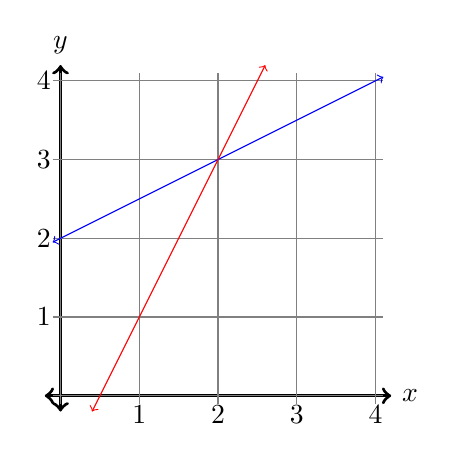
\begin{tikzpicture}
        \draw[very thick,<->] (-.2,0) -- (4.2,0) node[anchor=west] {$x$};
        \draw[very thick,<->] (0,-.2) -- (0,4.2) node[anchor=south] {$y$};
        \draw[gray,thin] (-.1,-.1) grid (4.1,4.1);
        \draw[blue,<->] plot[domain=-.1:4.1] (\x,.5*\x+2);
        \draw[red,<->] plot[domain=.4:2.6] (\x,2*\x-1);
        \foreach \x in {1,...,4} {
            \draw (\x,0) node[anchor=north] {$\x$};
            \draw (0,\x) node[anchor=east] {$\x$};
        }
    \end{tikzpicture}\end{center}
    The lines cross at the point $(2,3)$, so the solution is the $x$ value of this point: $x=2$.
    
    Next we solve symbolically/algebraically.
    \begin{align*}
        2x-1&=\frac{1}{2}x+2\\
        2x-\frac{1}{2}x-1&=2\\
        2x-\frac{1}{2}x&=2+1\\
        \frac{3}{2}x&=3\\
        x&=3\cdot\frac{2}{3}\\
        &=2.
    \end{align*}
    We got the same solution graphically and symbolically, $x=2$.
\end{solution}

\subsubsection{More complicated solutions}

So far, the equations we've see have all had solutions. In general, this doesn't always happen. There are three possiblilities for linear equations.
\begin{definition}{(Types of linear equation)}{def:types_of_linear_equation}
    There are three types of linear equation:
    \begin{itemize}
        \item Conditional equation: an equation with a single solution. Can be simplified to the form $x=a$ for some $a$.\\
        The equations we've seen so far have been conditional.
        \item Contradiction: an equation with no solutions.\\
        An equation is a contradiction if, when simplifying, you end up with a false statement such as $0=1$.
        \item Identity: an equation with infinitely many solutions.\\
        An equation is an identity if, when simplifying, you end up with a statement that is always true, like $0=0$ or $2x=2x$.
    \end{itemize}
\end{definition}

\begin{example}{(Textbook 2.2 ex 6)}{ex:2.2.6}
    Identify each equation as a contradiction, conditional equation, or identity.
    \begin{problem}
        \item $7+6x=2(3x+1)$
        \item $2x-5=3-(1+2x)$
        \item $2(5-x)-25=3(x-5)-5x$
    \end{problem}
\end{example}
\begin{solution}
    \begin{problem}
        \item We try to solve for $x$:
        \begin{align*}
            7+6x&=2(3x+1)\\
            7+6x&=6x+2\\
            7&=2.
        \end{align*}
        This is never true, so this equation is a contradiction.
        \item \begin{align*}
            2x-5&=3-(1+2x)\\
            2x-5&=3-1-2x\\
            4x-5&=2\\
            4x&=7\\
            x&=\frac{7}{4}.
        \end{align*}
        This is a single solution for $x$, so this equation is a conditional equation.
        \item \begin{align*}
            2(5-x)-25&=3(x-5)-5x\\
            10-2x-25&=3x-15-5x\\
            -2x-15&=-2x-15
        \end{align*}
        Since this is always true, this equation is an identity.
    \end{problem}
\end{solution}
% \includegraphics[width=6.5in]{Textbook_Mandatory_Examples/Exam1/2.2/2.2.6.png}

We can use the same operations we used for an equation of 1 variable to work with equations that have multiple variables. We isolate the variable of interest to express it in terms of the other variables.

\begin{example}{(Textbook 2.2 ex 12)}{ex:2.2.12}
    The area of a trapezoid with bases $a$ and $b$ and height $h$ is given by $a=\frac{1}{2}h(a+b)$. Solve this equation for $b$.
\end{example}
\begin{solution}
    We want to perform our allowed algebraic manipulations to get $b$ on one side.
    \begin{align*}
        A&=\frac{1}{2}h(a+b)\\
        2A&=h(a+b) && \text{multiply both sides by $2$}\\
        \frac{2A}{h}&=a+b && \text{divide both sides by $h$}\\
        \frac{2A}{h}-a&=b && \text{subtract $a$ from both sides}
    \end{align*}
    Now we have $b$ by itself on one side, so we have solved for $b$ in terms of the other variables.
\end{solution}
% \includegraphics[width=6.5in]{Textbook_Mandatory_Examples/Exam1/2.2/2.2.12.png}

\subsubsection{Word problems}

Now let's look at some examples using linear equations.

\begin{example}{(Textbook 2.2 ex 15)}{ex:2.2.15}
    A person 6 feet tall stands 17 feet from the base of a streetlight. If the person's shadow is 8 feet, estimate the height of the streetlight.
\end{example}
\begin{solution}
    \begin{minipage}{.36\textwidth}
        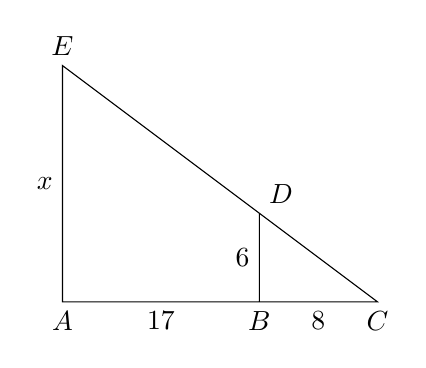
\begin{tikzpicture}
            \draw (2.5,0) node[anchor=north] {$B$} 
                -- node[below] {$8$} (4,0) node[anchor=north] {$C$}
                -- (2.5,4.5/4) node[anchor=south west] {$D$}
                -- (0,3) node[anchor=south] {$E$}
                -- node[left] {$x$} (0,0) node[anchor=north] {$A$}
                -- node[below] {$17$} (2.5,0) -- node[left] {$6$} (2.5,1.125);
        \end{tikzpicture}
    \end{minipage}
    \begin{minipage}{.63\textwidth}
        Let's begin by drawing a picture. We have two similar triangles:, as in the picture; the ratio of their base and horizontal sides will be the same, which we will use to find $x$.

        Since the ratio of the sides is the same, we know that \[\frac{6}{8}=\frac{x}{8+17}.\] Now we solve for $x$:
        \begin{align*}
            \frac{x}{25}&=\frac{3}{4}\\
            x&=25\cdot\frac{3}{4}\\
            &=\frac{75}{4}.
        \end{align*}
        We conclude that the lamppost is $\frac{75}{4}=18.75$ feet tall.
    \end{minipage}
\end{solution}
% \includegraphics[width=6.5in]{Textbook_Mandatory_Examples/Exam1/2.2/2.2.15.png}

\begin{example}{(Textbook 2.2 ex 13)}{ex:2.2.13}
    A large pump can empty a tank of gasoline in $5$ hours, and a smaller pump can empty the same tank in $9$ hours. If both pumps are used to empty the tank, how long will it take?
\end{example}
\begin{solution}
    Let $t$ be the number of hours it takes both pumps to fill up the tank. We want to come up with an equation which will let us solve for $t$.

    Since the large pump takes $5$ hours to empty the tank, each hour it empties $\frac{1}{5}$ of the tank. In $t$ hours, it will empty $t\cdot\frac{1}{5}$ of the tank.

    Similarly, since the small pump takes $9$ hours to empty the tank, each hour it empties $\frac{1}{9}$ of the tank and so in $t$ hours it empties $t\cdot\frac{1}{9}$ of the tank.

    Together, they empty the entire tank, which as a fraction is $\frac{1}{1}$. Therefore, we get the equation \[\frac{t}{5}+\frac{t}{9}=1.\]

    Now we solve for $t$:
    \begin{align*}
        \frac{t}{5}\cdot\frac{9}{9}+\frac{t}{9}\cdot\frac{5}{5}&=1\\
        \frac{9t}{45}+\frac{5t}{45}&=1\\
        \frac{14t}{45}&=1\\
        t&=\frac{45}{14}.
    \end{align*}
    Therefore, it takes $\frac{45}{14}\approx3.21$ hours for both pumps working together to empty the tank.
\end{solution}
% \includegraphics[width=6.5in]{Textbook_Mandatory_Examples/Exam1/2.2/2.2.13.png}

\begin{directions}
    Bonus example; do as time permits. Also, advise students that examples 14 and 16 in the book are worked examples of word problems that they can reference.
\end{directions}
\begin{example}{}{ex:density_linear_equation}
    Crushed sandstone has a density of 2.1 metric tons per meter cubed, while fill sand has a density of 1.4 metric tons per meter cubed. What percentage fill sand should you mix with crushed sandstone to get a fill material with a density of 1.5 tons per meter cubed?
\end{example}
\begin{solution}
    Let $x$ be the fraction of the mix that is fill sand. Then $1-x$ of the mix is crushed sandstone. Per 1 cubic meter of the mix, we have $x$ cubic meters of fill sand and $1-x$ cubic meters of crushed sandstone. Based on the densities of the materials, this will weigh \[x\cdot 1.4 + (1-x)\cdot2.1\text{ metric tons.}\]

    Since this is 1 cubic meter of material, we need it to weight $1.5$ metric tons. This gives us the equation \[1.4x+2.1(1-x)=1.5.\]

    Now we solve for $x$:
    \begin{align*}
        1.4x+2.1(1-x)&=1.5\\
        1.4x+2.1-2.1x&=1.5\\
        -.7x+2.1&=1.5\\
        -.7x&=-.6\\
        x&=\frac{.6}{.7}\\
        &=\frac{6}{7}.
    \end{align*}
    Now we know what fraction of the mix is fill sand; we want to convert this to a percentage. As a decimal, $\frac{6}{7}=.\overline{857142}$, so as a percent this is approximately $85.71\%$ of the mixture.
\end{solution}

\end{document}

\documentclass{article}
\usepackage[print]{notes}

\begin{document}

\setcounter{section}{2}
\setcounter{subsection}{2}

\subsection{Linear Inequalities}

Previously, we have worked with linear equations. Now we will look at linear inequalities.

\begin{definition}{(Inequality)}{def:inequality}
    Recall than an equation is two quantities related with $=$.

    An inequality is two quantities related by one of:
    \begin{itemize}
        \item $<$ means left is strictly less than right side
        \item $\leq$ means left is less than or equal to right
        \item $>$ means left is strictly greater than right
        \item $\geq$ means left is greater than or equal to right
    \end{itemize}
\end{definition}

We are allowed to do certain things when working with inequalities:

\begin{process}{Symbolically manipulating inequalities}{process:inequalities}
    We are allowed to do certain things when working with inequalities:
    \begin{itemize}
        \item Simplify the expression on either side of the inequality sign\\Ex: if $3(x-1)\leq 5$, we can distribute to simply the left: $3x-1\leq 5$.
        \item Add or subtract something from both sides\\Ex: if $x-5>17$, we can add 5 to both sides to get $x>17+5$.
        \item Multiply or divide both sides by a positive number\\Ex: if $2x<16$, we can divide both sides by 2 to get $x<8$.
        \item Multiply or divide both sides by a negative number, {\bf and flip the sign}\\Ex: if $-\frac{1}{3}x\leq 1$, then we can multiply both sides by $-3$ and flip the sign to get $x\geq -3$.\\We have to flip the sign in order to keep the statement true. For example, $-1>-5$ but if we multiply both sides by $-1$ and don't flip the sign we get $1>5$ which is false.
        \item Replace something with something else that is equal to it\\Ex: if we have $x \geq a$ and know $a=3$, we can replace $a$ with $3$ to get $x\geq3$.
    \end{itemize}
\end{process}

\begin{remark}{}{rmk:switch_sides_inequality}
    We can always rewrite an inequality to use $<$ instead of $>$ or $\leq$ instead of $\geq$ by switching the sides.
\end{remark}

\begin{definition}{(Bounds)}{def:bounds}
    \begin{itemize}
        \item If $a<x$ or $a\leq x$, we say that $a$ is a lower bound for $x$
        \item If $x<b$ or $x\leq b$, we say that $b$ is an upper bound for $x$
    \end{itemize}
\end{definition}

\begin{definition}{(Linear inequality)}{def:linear_inequality}
    A linear inequality is an inequality that can be rearranged to look like $ax+b>0$ or $ax+b\geq 0$.

    Another way to think about this is that it's a statement like we had for linear equations, but with an inequality sign instead of an equals sign.
\end{definition}

\begin{definition}{(Linear inequality)}{def:linear_inequality}
    A linear inequality is an inequality that can be rearranged to look like $ax+b>0$ or $ax+b\geq 0$.

    Another way to think about this is that it's a statement like we had for linear equations, but with an inequality sign instead of an equals sign.
\end{definition}

\includegraphics[width=6.5in]{Textbook_Mandatory_Examples/Exam2/2.3/2.3.1.png}

\begin{definition}{}{def:three_part_inequality}
    A three-part inequality is one with both an upper bound and lower bound on a quantity. 

    Alternatively, we can think of a three-part inequality as having two inequality signs which must ``point'' the same way.
\end{definition}

\begin{example}{}{ex:three_part_inequalities}
    Determine which of the following are valid 3-part inequalities:
    \begin{problem}
        \item $5 > 3 \geq x$
        \item $2 < x \geq 4$
        \item $a < x < b$
    \end{problem}
\end{example}
\begin{solution}
    \begin{problem}
        \item This is a valid three-part inequality because the middle term has one lower bound and one upper bound. We could write it in one of the four forms by reversing it: $x\leq 3 < 5$.
        \item This is not a valid three-part inequality because the middle term has two lower bounds and no upper bound.
        \item This is a valid three-part inequality.
    \end{problem}
\end{solution}

\begin{remark}{}{rmk:inequality_from_interval}
    Previously, we've looked at interval notation. We learned how to write an interval from a three part inequality where the middle term is $x$, or from a two-part inequality where one side is $x$. Similarly, an interval gives us an inequality.
\end{remark}

\includegraphics[width=6.5in]{Textbook_Mandatory_Examples/Exam2/2.3/2.3.6.png}

Just like we can solve linear equations graphically, we can also solve linear inequalities graphically. To do this, we treat each side of the inequality as a linear function and graph them.

\includegraphics[width=6.5in]{Textbook_Mandatory_Examples/Exam2/2.3/2.3.2.png}

We can also do word problems with linear inequalities. This is often useful when we care about a range of results, not just one specific value.

\includegraphics[width=6.5in]{Textbook_Mandatory_Examples/Exam2/2.3/2.3.7.png}

\setcounter{section}{2}
\setcounter{subsection}{3}
\setcounter{subsubsection}{4}

\subsubsection{Inequality word problems}

\markright{2.3 (Interlude) Modeling with linear inequalities}

\begin{process}{Solving (in)equality word problems}{}
    \begin{enumerate}
        \item Write a (linear) equation to model the situation
        \item Determine the inequality that gives us the desired solution, using your equation
        \item Solve the inequality
    \end{enumerate}
\end{process}

\begin{example}{}{}
    A car starts with 12 gallons of gas. Driving 25 miles takes 1 gallon of gas. How far can it drive and still have at least 6 gallons of gas left?
\end{example}

\begin{solution}
    \begin{enumerate}
        \item Equation modeling the situation:
        
        The independent variable here ($x$) is number of miles driven, and the dependent variable ($y$) is gallons of gas the car has left. We want to write a function that tells us how many gallons of gas the car has left after driving $x$ miles.

        The initial value is $f(0)=12$ gallons of gas.

        The rate of change/slope should be change in $y$ over change in $x$. We know that driving 25 miles ($\Delta x=25$) takes 1 gallon of gas ($\Delta y=-1$; this is negative since the car has 1 gallon less of gas afterwards). Thus, the rate of change is $\frac{-1}{25}$.

        Putting this together, we get $f(x)=-\frac{1}{25}x+12$.
        \item Inequality for what we're solving for:
        
        We want the car to have at least 6 gallons of gas, so $f(x)\geq 6$. Plugging in our formula for $f(x)$, this means $-\frac{1}{25}x+12\geq 6$.

        \item Solve:
        \begin{align*}
            -\frac{1}{25}x+12&\geq 6\\
            -\frac{1}{25}x&\geq -6\\
            x\;&\boxed{\leq}-6\cdot -25\\
            x&\leq 150.
        \end{align*}
        Therefore, the car can drive up to 150 miles and still have at least 6 gallons of gas.
    \end{enumerate}
\end{solution}

\begin{example}{}{}
    A biker is 50 miles from home. She bikes towards home 15 miles per hour. When will she be at most 10 miles from home? 
\end{example}

\begin{solution}
    \begin{enumerate}
        \item Independent variable is time (this is always a good guess for situations involving position/speed!)
        
        Dependent variable is distance from home.

        Initial value is initial distance from home, $50$ (miles).

        Rate of change is $-15$ since the distance between the biker and her home is decreasing at 15 miles per hour.

        All together, this gives us $f(x)=-15x+50$.
        \item We want her to be at most 10 miles from home; $f(x)\leq 10$. Plugging in our formula for $f(x)$ gives us $-15x+50\leq 10$.
        \item \begin{align*}
            -15x+50&\leq 10\\
            -15x&\leq-40\\
            x&\geq\frac{-40}{-15}=\frac{8}{3}
        \end{align*}
        So, at any time after 2 hours and 40 minutes, she will be at most 10 miles from home.
    \end{enumerate}
\end{solution}

\end{document}

\documentclass{article}
\usepackage{notes}

\begin{document}

\setcounter{section}{2}
\setcounter{subsection}{3}

\subsection{Modeling with linear functions}

In science, we often talk about dependent and independent variables. In an experiment, we change the value of an independent variable and then observe the effect on the dependent variable.
A function can be used to represent this sort of relationship. The independent variable is our input variable $x$, and the dependent variable is the resulting value of the function, $f(x)$.

Sometimes, the dependent variable will change at a constant rate with respect to the independent variable. Then we can model these situations with a line.

\includegraphics[width=6.5in]{Textbook_Mandatory_Examples/Exam2/2.4/2.4.1.png}

Domain is only $[0,3]$ or $\{0,1,2,3\}$ since prediction only good through 2018, and we generally don't think about fractional years.

Domain is only $[0,5]$ because we can't keep slowing down after stopping*.

\includegraphics[width=6.5in]{Textbook_Mandatory_Examples/Exam2/2.4/2.4.3.png}

One area where linear equations as models regularly come up is physics.

\begin{thm}{(Hooke's law)}{thm:hooke}
    Hooke's law is a theorem of physics which tells us that the distance a spring stretches is proportional to the force applied to the spring. The presentation our book uses is \[F=kx\] where $F$ is the weight (in pounds) of an object hung from the spring, $k$ is the spring constant for that spring, and $x$ is the distance (in inches) that the spring stretches.
\end{thm}

\includegraphics[width=6.5in]{Textbook_Mandatory_Examples/Exam2/2.4/2.4.6.png}

Sometimes, there isn't a single formula that works to describe all of a situation. In this case, we can combine multiple formulas which describe parts of the data using a piecewise function.

\begin{definition}{(Piecewise function)}{def:piecewise}
    A piecewise function combines multiple formulas that describe what happens in different parts of the domain. We write piecewise functions like \[f(x)=\begin{cases}\text{formula 1}&\text{domain 1}\\\text{formula 2}&\text{domain 2}\\\quad\;\vdots&\;\quad\vdots\end{cases}\]
\end{definition}

\begin{example}{(Floor function)}{ex:floor_fct}
    One example of a piecewise function is the floor function (your book calls this the greatest integer function). This function takes in a number and returns the greatest integer less than or equal to that number. In essence, it ``rounds down'' to the nearest whole number. We can write this like \[\lfloor x\rfloor=\bigl\{\;n\qquad n\leq x<n+1 \text{ and $n$ is an integer}\bigr.\] This function formalizes the fact that sometimes we have things which we can't have a fractional quantity of, like students in a class or days in a month.
\end{example}

\includegraphics[width=6.5in]{Textbook_Mandatory_Examples/Exam2/2.4/2.4.5.png}

\end{document}

\end{document}